\chapter{Analiza wymagań i projekt systemu}
\section{Przegląd istniejących rozwiązań}
Aby dobrze sprecyzować wymagania, aplikacje wymienione we wstępie poddano głębszej analizie. 
Pozwoliła ona na zidentyfikowanie mocnych i słabych stron, które posłużyły jako inspiracja do stworzenia własnego systemu.
Wyniki tej analizy zamieszczono poniżej.
\subsection{BlaBlaCar}
BlaBlaCar to jedna z największych platform do organizowania wspólnych przejazdów na świecie. 
Umożliwia użytkownikom oferowanie i wyszukiwanie przejazdów, a także ocenianie kierowców i pasażerów. 
System ten charakteryzuje się intuicyjnym interfejsem użytkownika oraz szeroką bazą użytkowników, co zwiększa szanse na znalezienie odpowiedniego przejazdu. 
Jednakże, platforma ta ma również swoje wady, takie jak pobierane opłaty za korzystanie z usług oraz ograniczenia w 
zakresie dostępności w niektórych regionach (np.\ w Stanach Zjednoczonych). Ponadto, do wyników wyszukiwania przejazdów dodawane są oferty komunikacji zbiorowej,
takie jak autobusy czy pociągi. Może to wpłynąć na łatwość znalezienia przejazdu samochodem, który może być głównym celem użytkownika.
\subsection{InOneCar}
InOneCar to polska aplikacja do organizacji wspólnych przejazdów, głównie na Dolnym Śląsku.
Podobnie jak BlaBlaCar, umożliwia użytkownikom oferowanie i wyszukiwanie przejazdów, obliczanie kosztów i zarządzanie rezerwacjami na przejazdy. 
Jednakże, w przeciwieństwie do BlaBlaCar, InOneCar nie pobiera opłat za korzystanie z usług.
Problemem tej platformy jest brak swobody w oferowaniu przejazdów. Kierowcy mogą oferować przejazdy wyłącznie na trasach, które zostały wcześniej zdefiniowane
przez administratorów systemu. Jak wspomniano we wstępie, kryterium stworzenia ,,korytarza'' jest wystarczająca liczba zgłoszeń kierowców i pasażerów na danej trasie. 
W przypadku braku wystarczającej liczby zgłoszeń, kierowcy nie mogą oferować przejazdów na tej trasie. Zdecydowanie ogranicza to swobodę kierowców w oferowaniu przejazdów
na mało popularnych trasach, co pogarsza sytuację wykluczenia komunikacyjnego w mniejszych miejscowościach.
\section{Analiza wymagań funkcjonalnych i niefunkcjonalnych}
Aplikacja pozwala użytkownikom na oferowanie i wyszukiwanie przejazdów oraz zarządzanie rezerwacjami na przejazdy. 
W tym celu wyszczególniono 2 główne role w procesie korzystania z aplikacji: kierowcę i pasażera. 

Poza wyznaczeniem punktów startu i końca przejazdu oraz planowanej daty i godziny odjazdu, kierowca może przyjmować rezerwacje miejsc w swoim samochodzie od pasażerów.
Aby ograniczyć liczbę rezerwacji, jaką kierowca może zaakceptować na daną ofertę przejazdu, kierowca musi podać liczbę wolnych miejsc w aucie. 
Kierowca musi również określić podstawowe dane dotyczące swojego pojazdu, takie jak ogólny opis (np.\ model, marka, kolor), 
numer rejestracyjny oraz uśrednione spalanie paliwa, wykorzystywane do propozycji podziału kosztów przejazdu.

Sam pasażer, podobnie jak kierowca, określa punkt na mapie i promień, wokół którego ma być wyszukiwana oferta przejazdu, punkt docelowy, oraz planowaną datę odjazdu.
Aplikacja znajduje najlepiej dopasowaną ofertę przejazdu, a następnie pozwala pasażerowi na dokonanie rezerwacji miejsca w samochodzie kierowcy.
Po złożeniu rezerwacji, kierowca może ją zaakceptować lub odrzucić. W obu przypadkach, pasażer widzi aktualny status swojej rezerwacji w aplikacji. 
W przypadku akceptacji rezerwacji, pasażer otrzymuje dane kontaktowe do kierowcy.
\subsection{Diagram wymagań SysML}
Na podstawie powyższego opisu stworzono diagram wymagań za pomocą języka PlantUML. 
Wyodrębniono w nim 2 aktorów: kierowcę i pasażera. Kierowca jest powiązany z wymaganiami dotyczącymi tworzenia ofert przejazdów oraz tworzenia rezerwacji, 
natomiast pasażer z wymaganiami dotyczącymi wyszukiwania przejazdów i tworzenia rezerwacji.
Poniższy diagram przedstawia wymagania funkcjonalne systemu, a także relacje między nimi.
% Na razie wstawione w ten sposób, nie wiem, czy je pomniejszyć czy przerysować w mermaid albo innym narzędziu i inaczej ustawić elementy
% Przy użyciu \usepackage{float} i opcji [H] tekst się bardzo rozjeżdża, 
% na razie zostawię jak jest a jak tekst rozdziału 2 będzie gotowy to wtedy się poprawi
\begin{figure}[h]
	\centering
	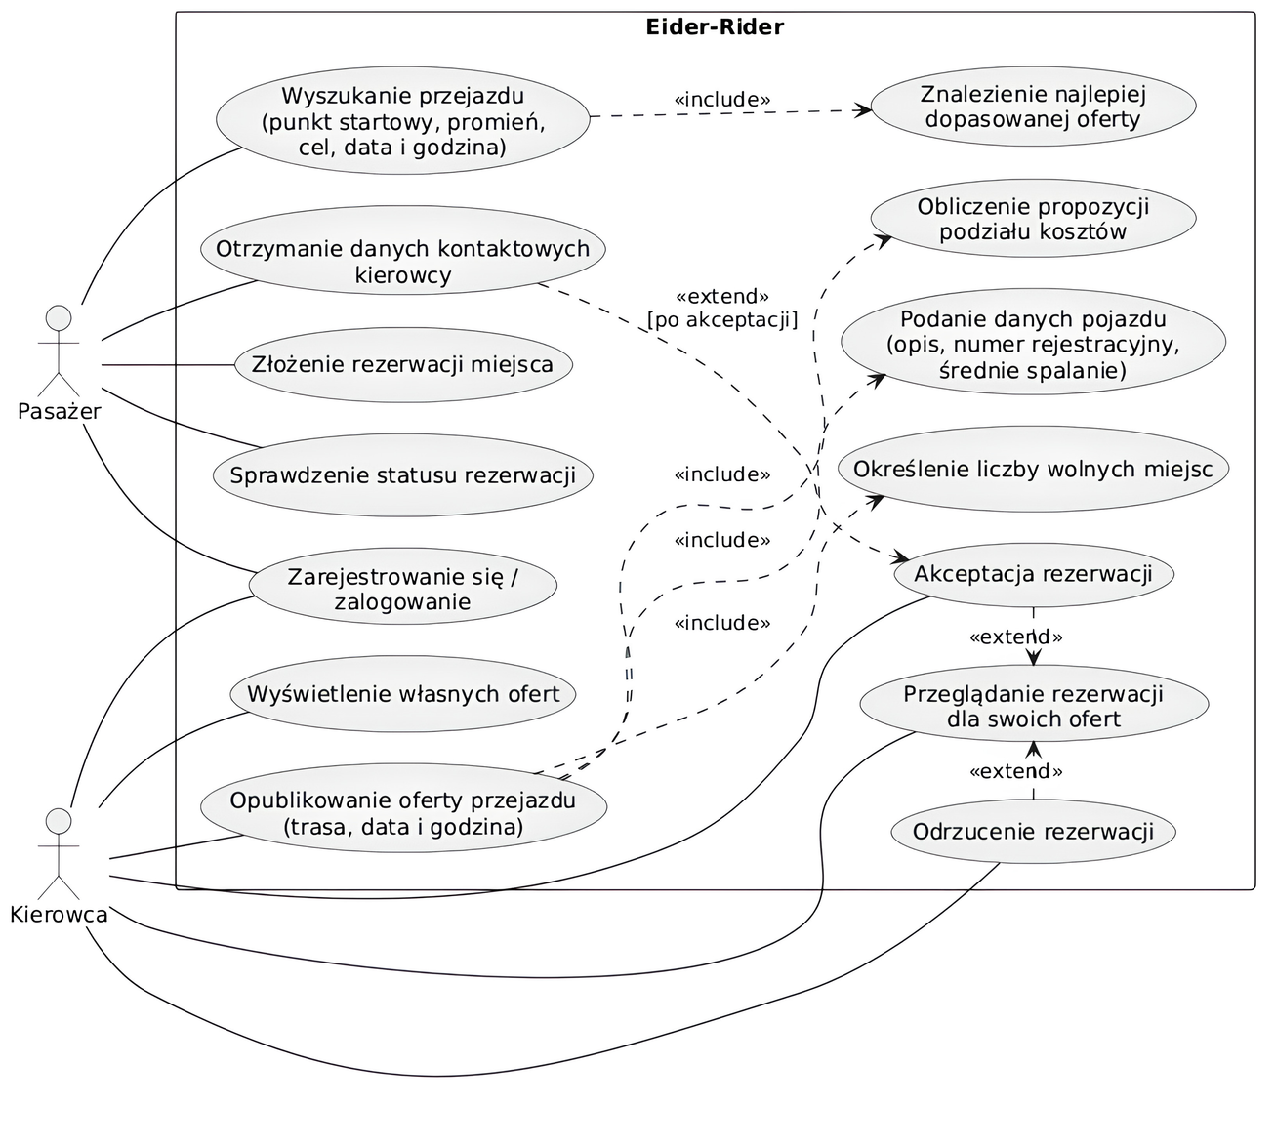
\includegraphics[width=0.7\linewidth]{rys02/Use_case_diagram_upscaled.pdf}
	\caption{Diagram wymagań systemu}
	\label{fig:requirements-diagram}
\end{figure}

\section{Architektura i projekt systemu}
System zaprojektowano w oparciu o architekturę klient-serwer, w której aplikacja internetowa pełni rolę klienta HTTP, a serwer obsługuje logikę biznesową i przechowuje dane w bazie danych.
Sam serwer został podzielony na kilka modułów, z których każdy odpowiada za określoną funkcjonalność systemu.

% TODO: dodać JWT do słownika i ew. poprawić opis w tekście
Wszystkie zapytania klienta HTTP do autoryzowanych punktów końcowych są uwierzytelniane za pomocą JWT (ang.~\emph{JSON Web Token}), 
który weryfikuje tożsamość użytkownika i jego uprawnienia do korzystania z wymaganych funkcji.

Pomiędzy modułem \emph{API} a modułem logiki biznesowej \emph{Core} znajduje się mediator, który ma na celu zmniejszenie sprzężenia między tymi modułami.
Mediator jest odpowiedzialny za przekazywanie żądań od punktów końcowych API do odpowiednich funkcji logiki biznesowej, a także za zwracanie wyników z powrotem do klienta.
Moduł Core zawiera wszystkie funkcje logiki biznesowej i serwisy, które są wykorzystywane przez kontrolery API. 
Posiada on 2 podmoduły: 
\begin {itemize}
    \item \emph{Core.Auth} - zawiera serwisy odpowiedzialne za autoryzację i uwierzytelnianie użytkowników,
    \item \emph{Core.Common} - zawiera używane w wielu miejscach wyjątki i klasy pomocnicze.
\end{itemize}

Komunikacja z bazą danych odbywa się za pomocą klas zdefiniowanych w module \emph{Persistence}.
Głównym zadaniem tego modułu jest definiowanie oraz mapowanie obiektów na tabele w bazie danych, generowanie danych testowych i wykonywanie migracji bazy danych.
% O szczegółach implementacji (bibliotekach, framework'u itp.) miałem zamiar napisać w rozdziale 3, 
% stąd brak terminów typowo .NET'owych ani wzmianek o wybranych technologiach w tym rozdziale.
\begin{figure}[h]
	\centering
	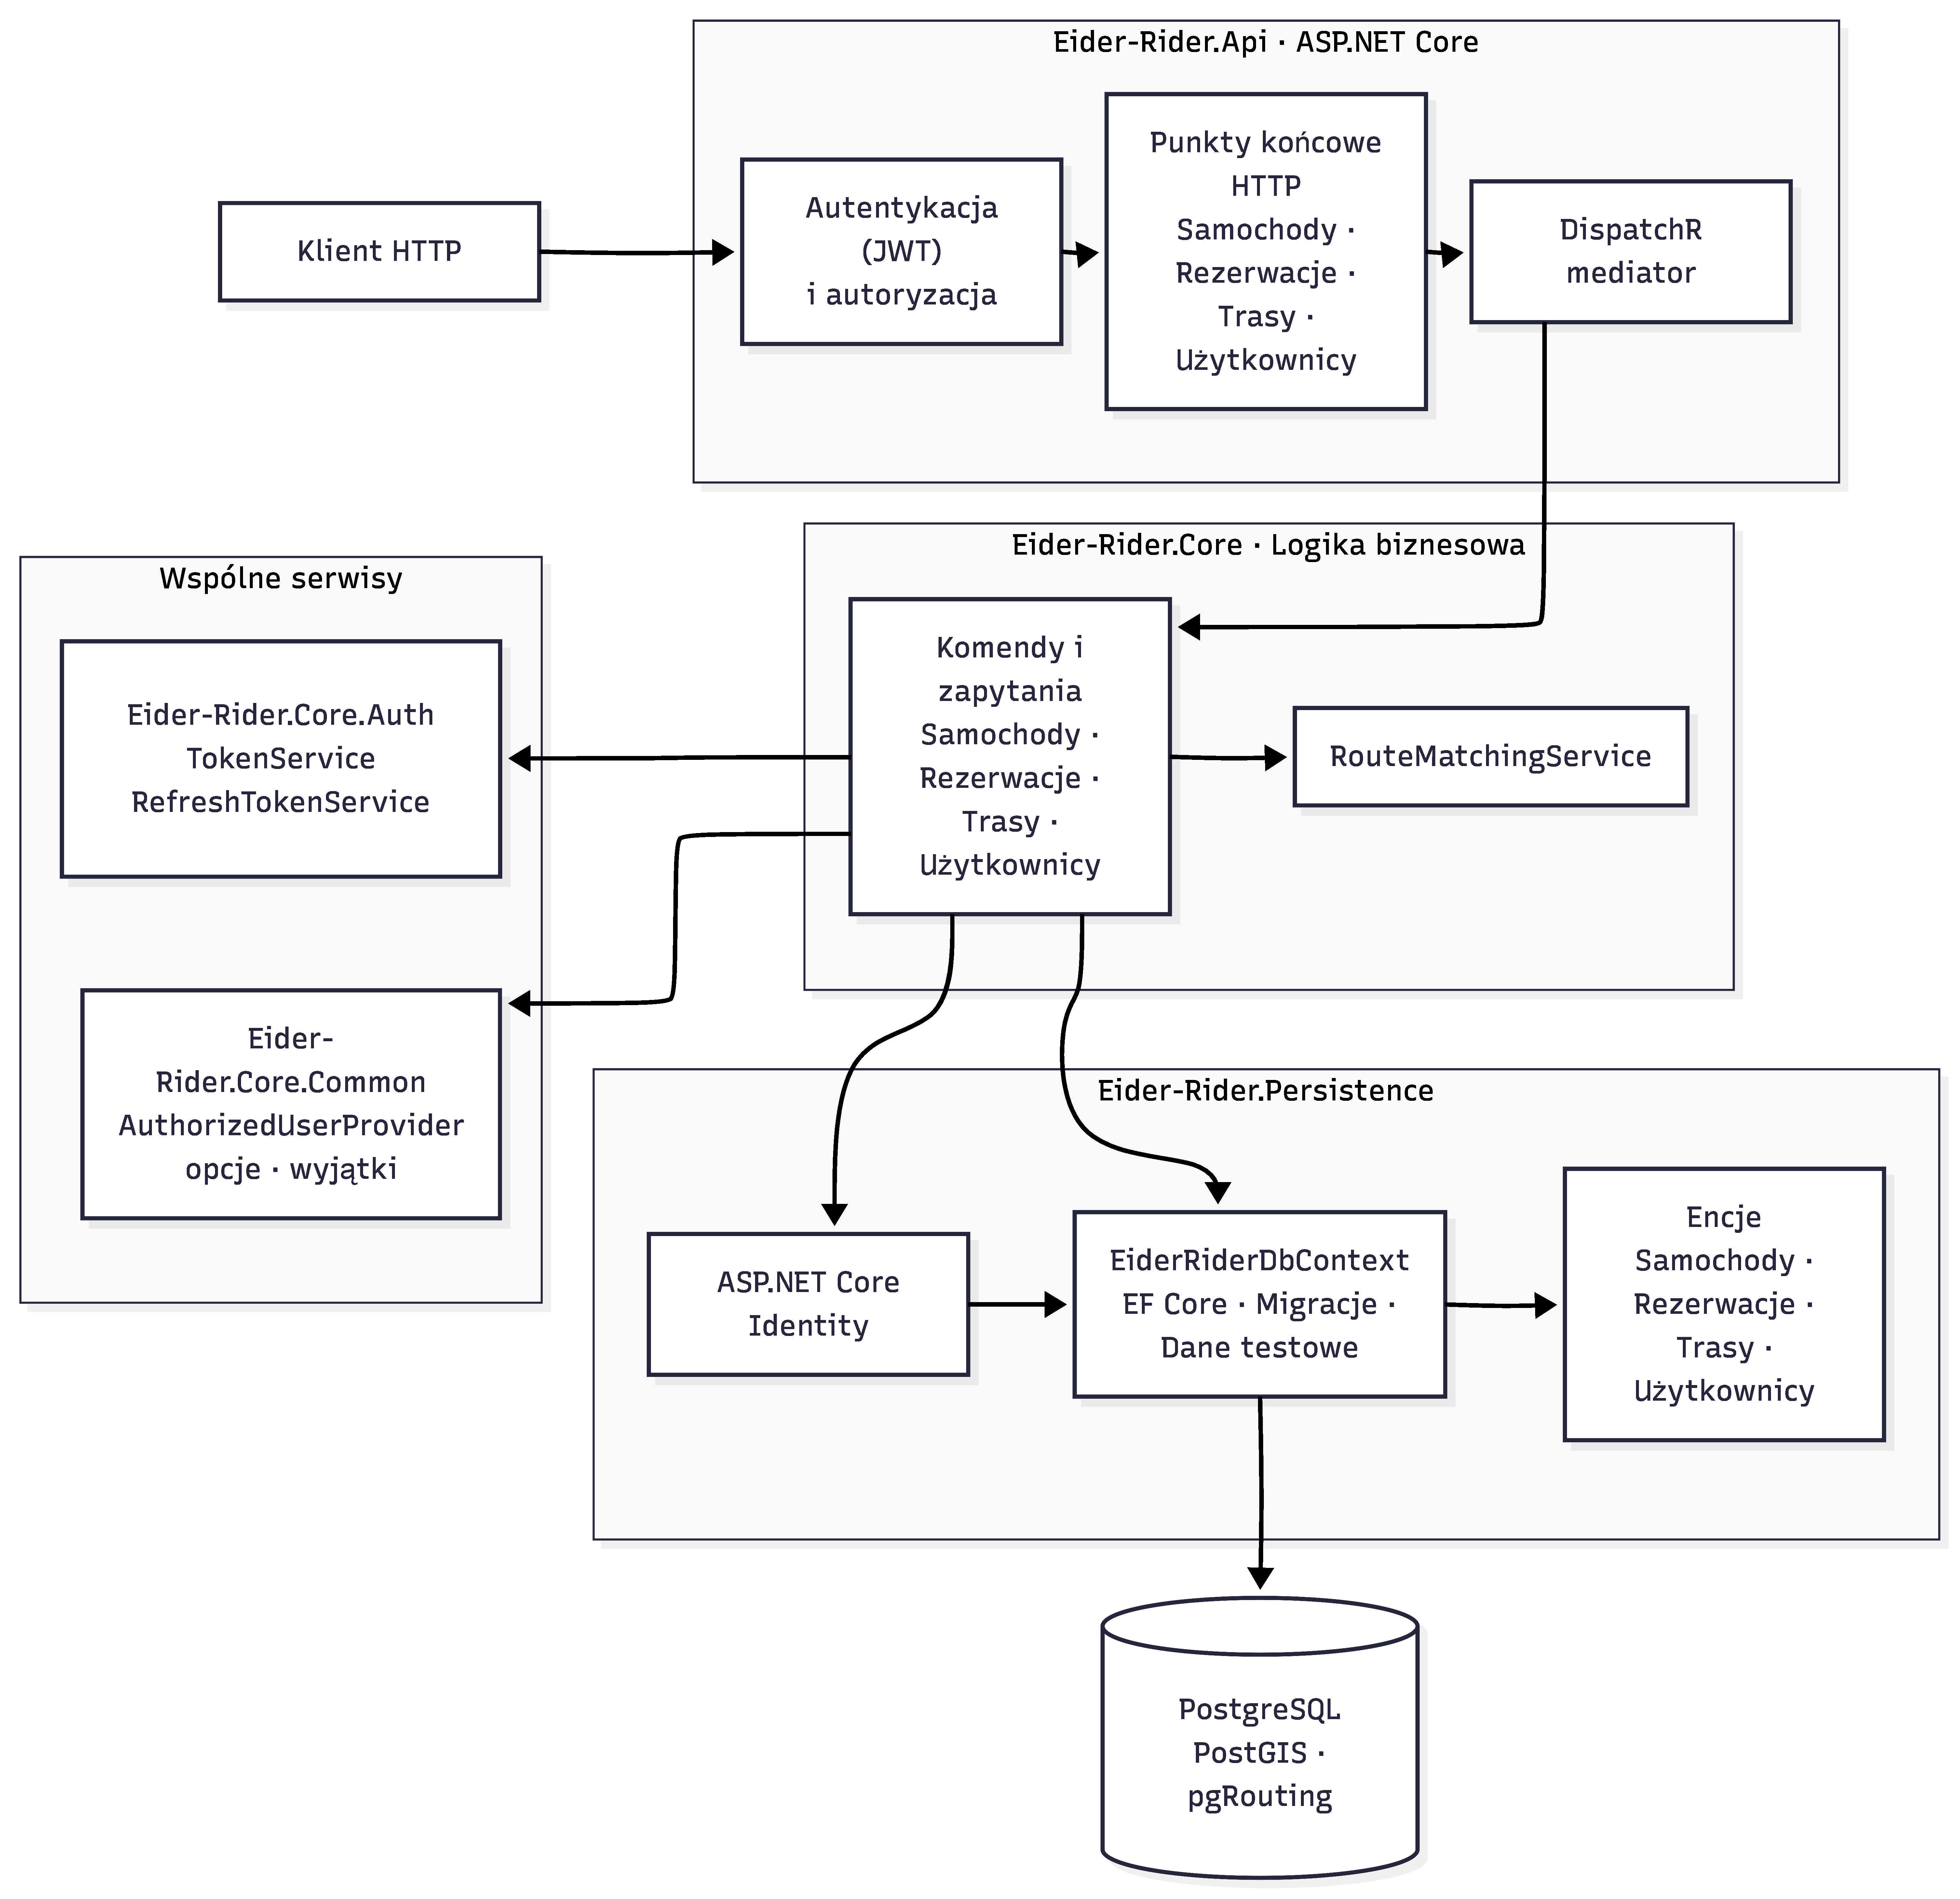
\includegraphics[width=0.9\linewidth]{rys02/Architecture_diagram_transparent.pdf}
	\caption{Diagram architektury systemu}
	\label{fig:architecture-diagram}
\end{figure}
\subsection{Model fizyczny bazy danych}
% Ze względu na charakter diagramu, czy nie lepsze będzie uwzględnienie go w rozdziale 3, w którym opisuję implementację?
Aby zrealizować wymagane funkcje systemu, zaprojektowano bazę danych, której model fizyczny przedstawiono na rysunku \ref{fig:entity-relationship-diagram}.
Składa się ona z 7 tabel, które przechowują informacje o użytkownikach, tokenach odświeżania, pojazdach, trasach i rezerwacjach.
Same encje oraz ich relacje zostały zdefiniowane w module \emph{Persistence} za pomocą ORM (ang.~\emph{Object-Relational Mapper}).
Dzięki mechanizmowi migracji, pozwala na automatyczne generowanie i aktualizowanie struktury tabel w bazie danych bezpośrednio na podstawie kodu źródłowego.
% Tutaj będę miał pytanie na konsultacjach co do tabel generowanych automatycznie przez framework, których na razie nie ma w diagramie.
\begin{figure}[h]
	\centering
	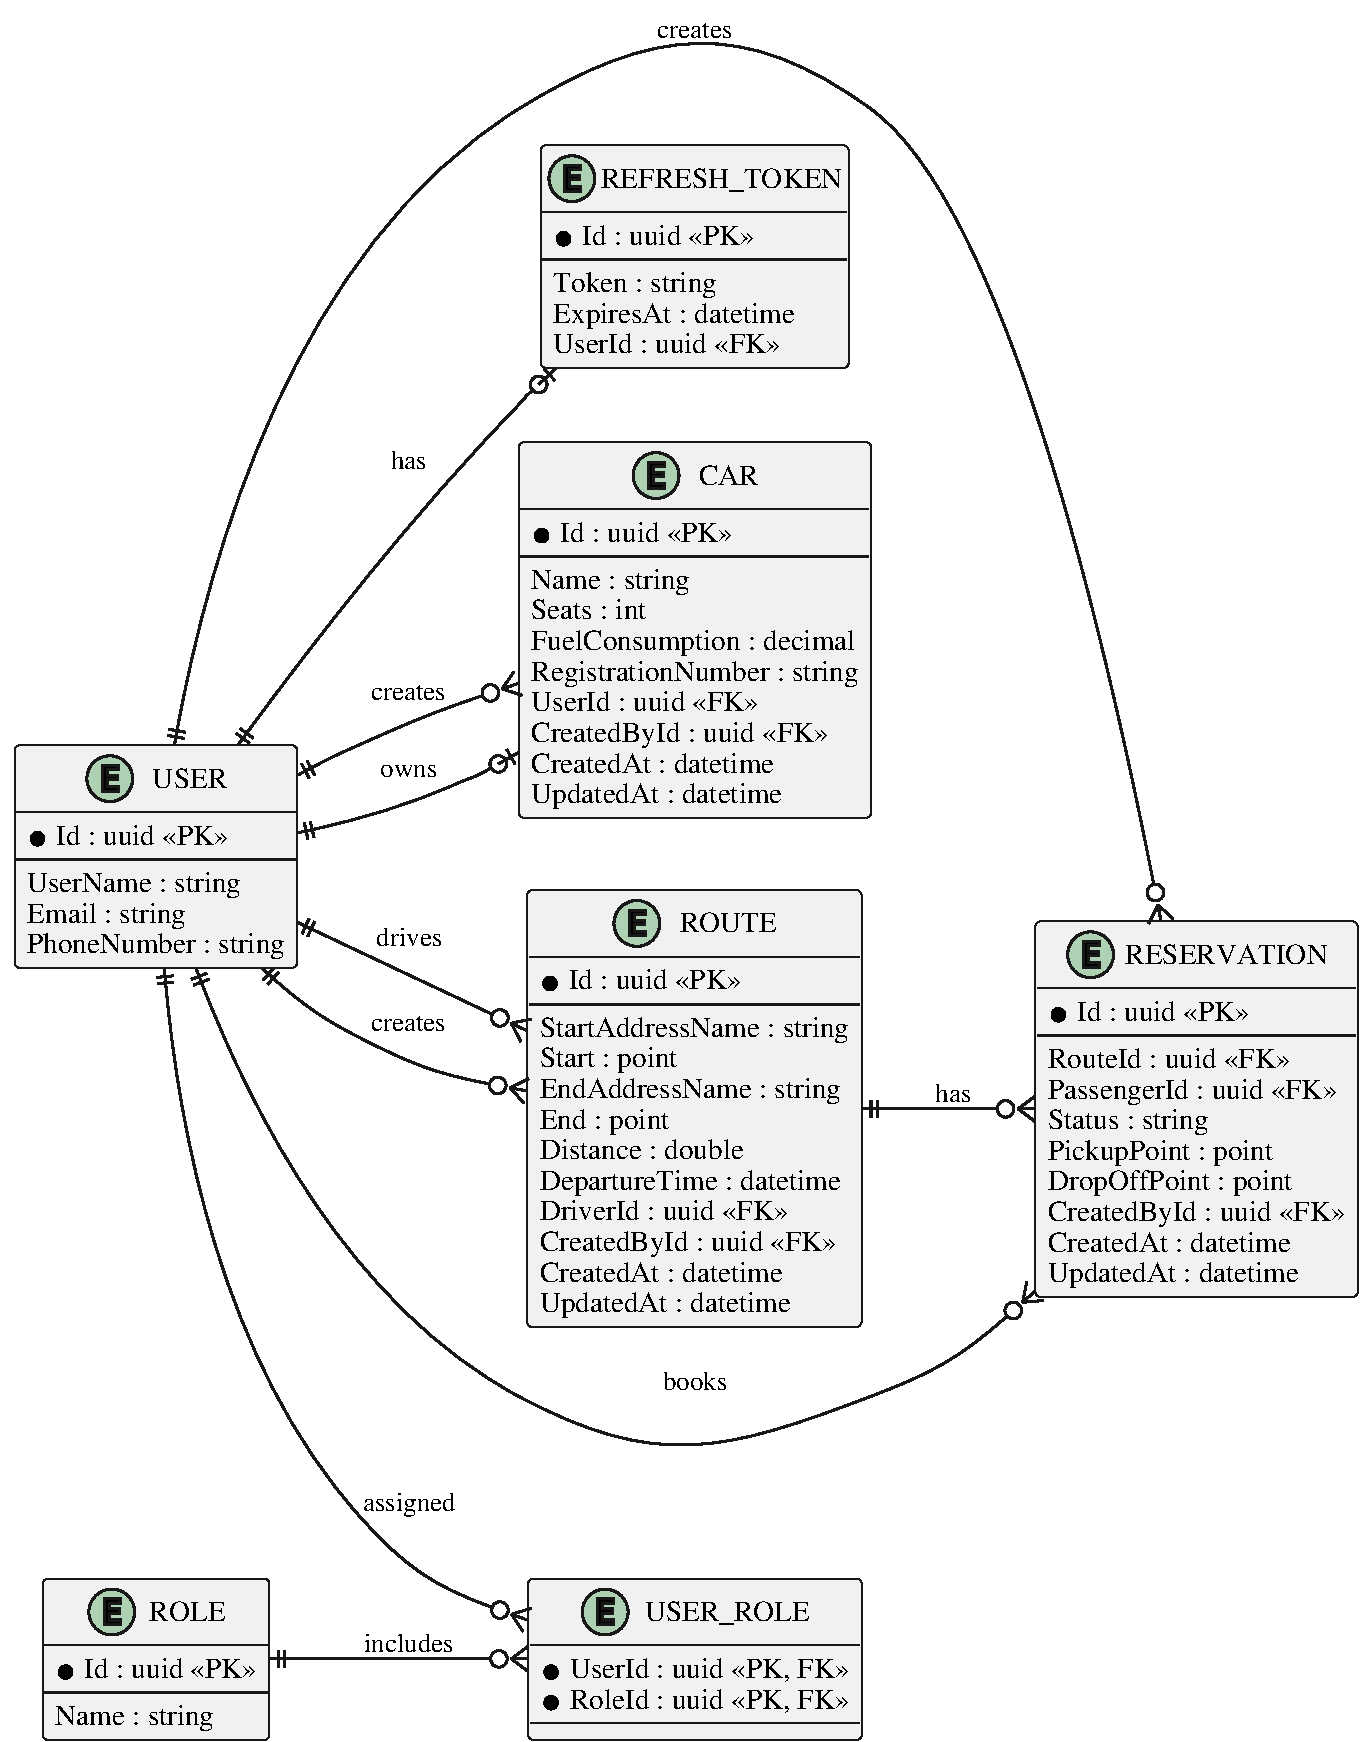
\includegraphics[width=0.8\linewidth]{rys02/Entity_relatioship_diagram.pdf}
	\caption{Diagram relacji encji w bazie danych}
	\label{fig:entity-relationship-diagram}
\end{figure}